\section{Bronwen}

\begin{center}
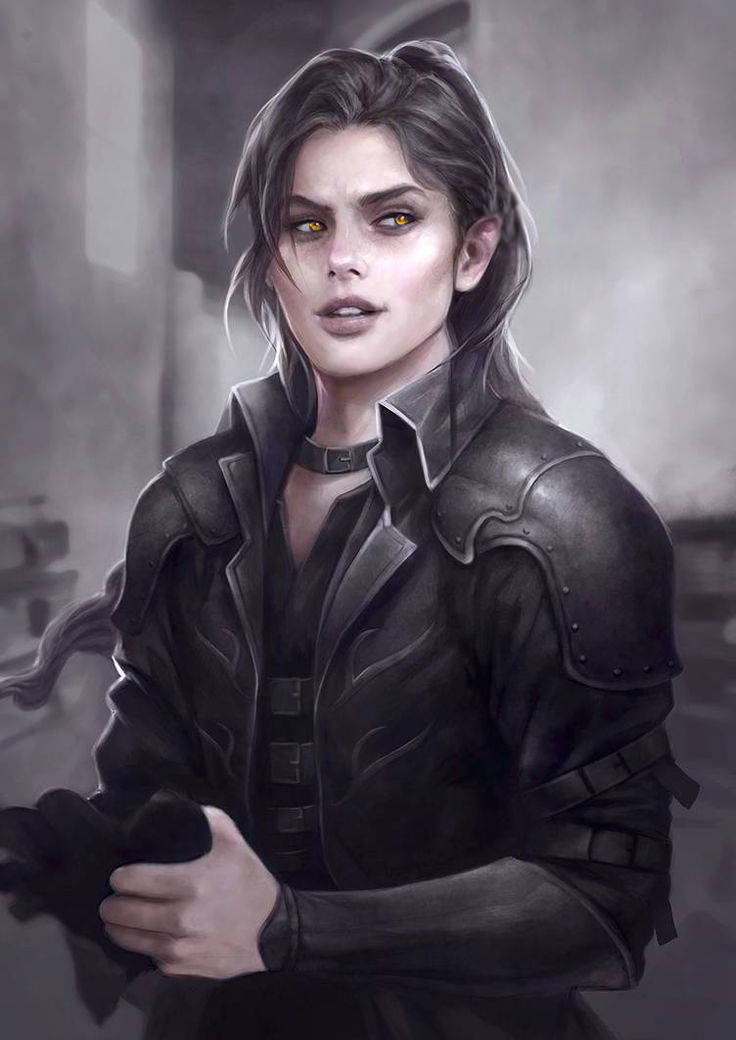
\includegraphics[width=80mm]{./content/img/bronwen_temp.png}
\begin{figure}[h]
\end{figure}
\end{center}

\subsection*{Details}

\noindent

Player: Jonathan Mann (after Exme's erasure) \\
Race: 	Devil \\
Class: 	Cleric (flying sword) \\
Age: 	Unknown \\
Status: Active

\subsubsection{Background}

Bronwen arrived after the destruction of Kalimar, at the point where the party had lost Exmerah and badly needed someone to keep them pointed in the right direction. She stood seven feet tall, with golden eyes and an incongruously warm Welsh accent, and she made no secret of being a creature of Hell. Lazarus had sent her, and the Empire of the Eight does not send minders to groups it has given up on.

\subsubsection{Personality and Traits}

For a devil, Bronwen was remarkably steady. She fought with a flying sword and mended the party's wounds when its luck ran out, playing the role of both enforcer and field medic. Her temperament ran calm and practical, a useful counterweight to a group that had just watched one of its own erase herself from existence.

Her most important talent was her command of darkness, which proved to be more than a battlefield trick. When the party was overwhelmed by the mass mind control of a mind flayer, it was Bronwen's darkness that broke the spell and freed them.

\subsubsection{Relationships}

Sent rather than chosen, Bronwen slotted into the party as Hell's representative, and the group came to rely on her where they had once relied on Exme's ingenuity and Burnie's experience. She kept Myron alive through the worst of the Nautiloid fighting, reviving him again and again, and her scrying gave the party their first clear look at the enemy: Canalon perched atop the guildmasters' hall in Hope's Rest, its many eyes turning to look straight back at her.

\subsubsection{Bronwen's Story}

Bronwen joined the remnant of the party for the final stretch of the campaign. She broke the Ulitharid's hold over the group during the boarding of the Nautiloid, kept Myron on his feet through the running battle that followed, and rode with the survivors aboard the Jecede railway to Hope's Rest. After Erin's death and Burnie's, when the survivors were moping and Burnie was smearing his own excrement on the walls in grief (the hook made it especially dangerous), it was Bronwen who snapped them out of it.  ``No more of that,'' she told them.  ``No more moping around, it's not helping anyone and more people are going to die.  The whole universe is relying on you to get your head in the bloody game.  Erin knew that.  Exme knew that.  And you all know it.''

When the party heisted the deserted Black Rock bank for the Armoury of Sin, Bronwen was among the handful still standing to help carry the gods' old war gear out of the vault.

\clearpage
